\documentclass{article}
\usepackage{graphicx}
\usepackage{amsmath}
\usepackage{acronym}
\usepackage{biblatex}

\title{Aposteriori Unimodality}
\author{Dimitris Tsirmpas, John Pavlopoulos}
\date{March 2025}


% Insert space after commas in math mode
\AtBeginDocument{%
  \mathchardef\stdcomma=\mathcode`,
  \mathcode`,="8000
}
\begingroup\lccode`~=`, \lowercase{\endgroup\def~}{\stdcomma\,}

\graphicspath{ {../graphs}  }
\bibliography{refs.bib}


\begin{document}

\maketitle

\section{Methodology}

\subsection{Problem Formulation}
\label{ssec:methodology:problem}

Let $\{c(d,1), c(d,2), \ldots\}$ be the comments\footnote{Also referred to as “dialogue turns” in some publications.} of a discussion $d$ and $A(d, i)$ be the set of annotations for comment $c(d, i)$. We assume that annotating a comment depends on three variables: its contents, the annotator's \ac{SDB}, and uncontrolled factors such as mood and personal experiences. Assuming that each comment is assigned multiple annotations from different annotators:
\begin{equation}
    A(d, i) = \{a(d, i, \theta) \mid i=1, 2, \ldots, \lvert d \rvert, \theta \in \Theta \}
\end{equation}
\noindent where  $a(d, i, \theta)$ is a single annotation for comment $c(d,i)$ and $\theta \in \Theta$ is the annotator's \ac{SDB}.

Since our goal is to pinpoint which specific characteristics contribute to polarization, we need a way to isolate individual attributes within a \ac{SDB}. By definition, $\theta$ is composed of multiple ``dimensions'' (e.g., age, sex, educational level) each of which is split between various groups. We can thus model $\theta$ as:
\begin{equation}
    \theta = \{(\xi_i, \mu) \mid i=1, 2, \ldots, k \mathpunct{,} g \in G_i\}
\end{equation} 
\noindent where $\Xi=\{\xi_1, \xi_2, \ldots, \xi_k\}$ is the set of \ac{SDB} dimensions, and $G_i$ is the set of possible groups for dimension $\xi_i$ (e.g., if $\xi_1$ corresponds to gender, then $G_1=\{\textit{male}, \textit{female}, \ldots\}$).


\subsection{Quantifying changes in polarization}
\label{ssec:methodology:polstat}

The mechanism defined in Section \ref{ssec:methodology:problem} allows us to isolate the effects of each \ac{SDB} dimension, but we still lack a mechanism with which to analyze that effect. In this section, we present the "pol-statistic" (polarization statistic) as a tool to not only attribute polarization to a dimension $\xi$, but also to specific groups within that dimension $g \in G_{\xi}$.

Intuitively, $\xi$ influences polarization within an annotation set when the annotations, divided according to each group $g \in G_{\xi}$, show greater polarization than the full set of annotations. For instance, consider a misogynistic comment in the context of an annotation task for bigoted speech (Figure~\ref{fig:ndfu_single_comment}). The annotations may be generally polarized, although annotations from female annotators might show low polarization (most may agree the comment is bigoted), and so may annotations from male annotators (but most may agree that it is \textit{not} bigoted). This suggests that the overall polarization is driven by disagreements between male and female annotators. 

\begin{figure}
	\centering
	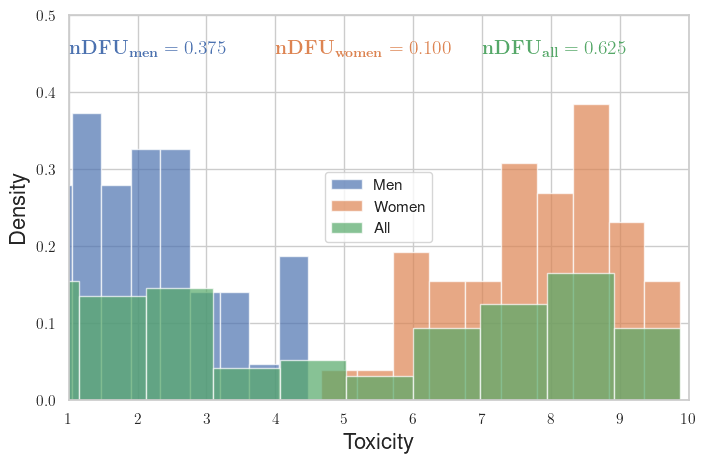
\includegraphics[width=0.8\linewidth]{ndfu_single_comment.png}
	\caption{Example where the whole annotation set is extremely polarized, but not when the annotations are split by group.}
	\label{fig:ndfu_single_comment}
\end{figure}

 However, directly using annotations for all comments in a discussion is not ideal because we can not control for factors like different comment content. For example, if women find one comment toxic more than men, and another much less toxic than men, the opposing effects might balance each other out, leading to a false negative. This effect is demonstrated in Figure~\ref{fig:ndfu_multi_comment}. To avoid this, we apply our statistic only within the same comment’s annotations instead. Thus, we can define our "pol-statistic" as:
\begin{equation}
	pol(c, \mu) = nDFU(A) - nDFU(P(A, \xi, g))
\end{equation}
\noindent where $P(A,\xi, g) = \{a(d, i, u) \in A | (\xi, \mu) \in \theta\}$ is the set of annotations $A$ for a comment $c(d, i)$ for which its annotators belong  to the group $g$ of \ac{SDB} dimension $\xi$.

\begin{figure}
	\centering
	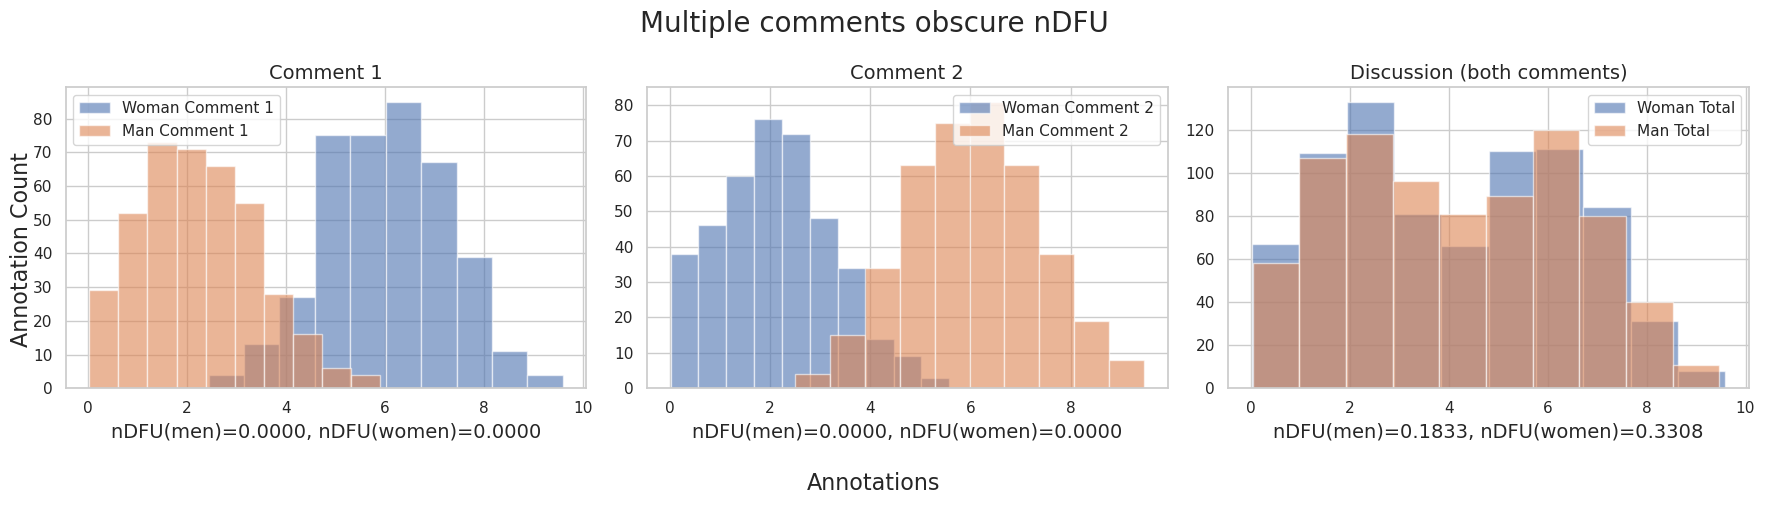
\includegraphics[width=\linewidth]{ndfu_multi_comments.png}
	\caption{Example where the opposite-directioned }
	\label{fig:ndfu_multi_comment}
\end{figure}



\subsection{The Aposteriori Unimodality Test}
\label{ssec:methodology:aposteriori}

Although intuitive, the \textit{pol statistic} can only be applied to individual comments, and is susceptible to inherent noise present in annotation tasks. If the polarization in a discussion $d$ is not driven by the attribute $\xi$, we would expect $pol(c, g) \approx 0,  \forall g \in G_{\xi}$. By obraining the pol statistics for all comments in a discussion $d$ we can apply a mean test with the null hypothesis :
\begin{equation}
	H_0: \frac{1}{\lvert d \rvert} \sum\limits_{c \in d} pol(c, g) = 0, \forall g \in G_{\xi}
\end{equation}
\noindent versus the alternative hypotheses: 
\begin{equation}
	H_i:  \frac{1}{\lvert d \rvert} \sum\limits_{c \in d}  pol(c, g_i) > 0, g_i \in G_{\xi}
\end{equation}

Since we are considering $\lvert G_{\xi} \rvert$ tests, we apply a multiple comparison correction to the resulting p-values. We choose the Bonferroni method \parencite{Bland170}, since it is widely used, generally conservative, and especially so towards correlated hypotheses \parencite{ChenFengYi2017}. The last point is important, since many annotation groups are likely to be inter-correlated (e.g., age categories such as 50-60 and 60-70 years). Furthermore, one of its largest weaknesses (large numbers-hundreds-of hypotheses) is unlikely to be met in annotation groups.

This procedure is referred to as the \textit{``Aposteriori Unimodality Test''}, where a small p-value suggests that we can not rule out that annotators of the $g$ group make a significant contribution to the overall annotator polarization.


\section{Acronyms}

\begin{acronym}[WWW]
    \acro{SDB}{SocioDemographic Background}
\end{acronym}

\printbibliography

\end{document}
